\chapter{Diseño del sistema}
\label{ch:diseno}
Tras haber realizado el análisis del sistema previamente, en este capítulo se desarrollan más en detalle las parte internas del mismo, como son las relacionadas con la arquitectura del sistema (\autoref{sec:arquitectura}), donde se define la manera en la que se relacionan y comunican las distintas partes que lo componen.

También se define la manera en la que se almacenan los datos (\autoref{sec:modelo}) y como son las interfaces que componen el sistema (\autoref{sec:interfaz}) con las que interactúa el usuario. 

Además, lo definido a continuación sienta la base para poder comenzar el desarrollo e implementación del sistema (\autoref{ch:implementacion}) y las pruebas que se realizan sobre el mismo (\autoref{ch:pruebas}).

\section{Arquitectura del Sistema}\label{sec:arquitectura}
El sistema que se desarrolla en este proyecto sigue un patrón de desarrollo bien definido, Modelo-Vista-Controlador~\cite{bucanek_model-view-controller_2009,hernandez_mvc_nodate}, que permite separar de una manera clara las diferentes partes del sistema que hay que desarrollar. Esta arquitectura se compone de las siguientes partes:
\begin{itemize}
	\item \textbf{Modelo:} Parte encargada de la representación lógica de la información en el sistema, los mecanismos para acceder a ella y almacenarla. Esta es la parte relacionada con la base de datos.
	\item \textbf{Vista:} Es la representación visual del sistema (interfaz web) que se muestra al usuario cuando utiliza la aplicación.
	\item \textbf{Controlador:} Representa toda la lógica del sistema, tanto el procesamiento de las medidas como el tratamiento de las peticiones al servidor.
\end{itemize}

Esta separación en tres partes permite que se puedan desarrollar e implementar las 3 partes en paralelo, de manera que quede todo más modularizado y dado el caso se puedan modificar o remplazar sin problema. Como podría ser, por ejemplo, que se quisiera cambiar la página web (vista) por otra diferente sin que haga falta modificar el modelo y controlador. 

Además, es ampliamente usado y se ha demostrado su eficacia en multitud de proyectos de software.
\pagebreak

En la \autoref{fig:mvc} se puede ver cuál es la relación entre las diferentes partes que lo componen, que son:
\begin{itemize}
	\item El usuario, en primer lugar, solicita al servidor que le mande la página web. Cuando este visualiza la web realiza solicitudes de servicios y contenidos que se van visualizando.
	\item El controlador recibe las solicitudes del usuario y se comunica con el módulo vista, para mandar la parte visual del sistema al usuario y que puede realizar más solicitudes. Cuando necesita acceder a información o almacenarla, se comunica con el modelo, para que este se encargue de hacerlo.
	\item El modelo se encarga de almacenar los datos y cuando se le solicite responde con los datos pedidos o los almacena en su caso.
	\item La vista envía, al usuario, la parte visual del sistema que le solicita el controlador, que es el que se encarga de la parte lógica de la web.
\end{itemize}

\begin{figure}[H]
	\ffigbox[\FBwidth]
	{\caption[Diagrama Modelo-Vista-Controlador]{Diagrama Modelo-Vista-Controlador~\cite{hernandez_mvc_nodate}}
		\label{fig:mvc}}
	{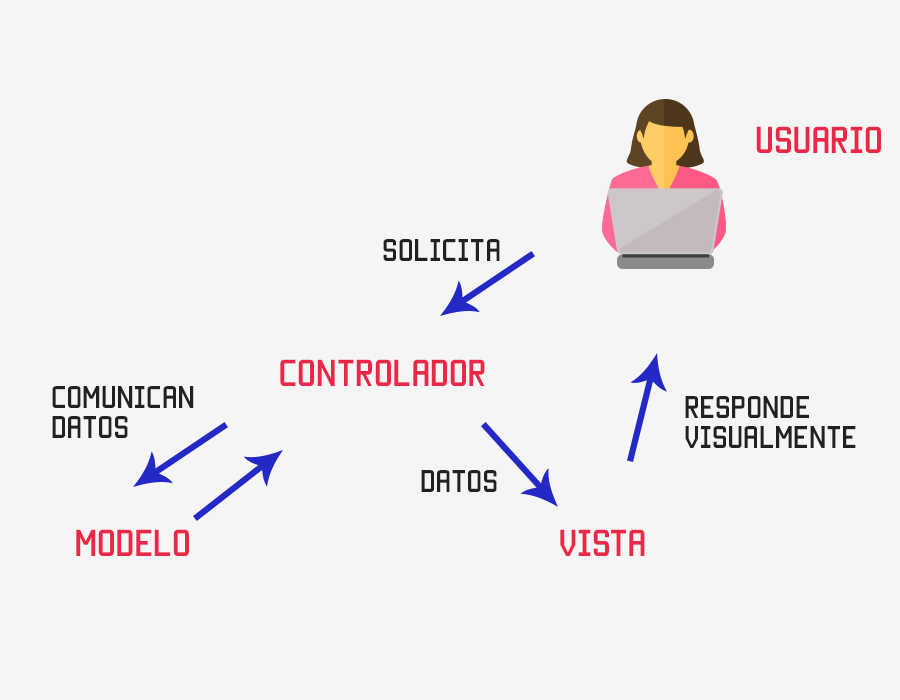
\includegraphics[scale=0.3]{mvc.jpg}}
\end{figure}

La manera en la que el usuario interactúa con el sistema es de Cliente-Servidor, lo que quiere decir que el usuario lo único que tiene que hacer para utilizar el sistema es conectarse y acceder. Es el servidor el que tiene todo el sistema y se encarga de responder a todas las peticiones, gestionando los dispositivos, datos y página web. 
\pagebreak

\section{Diagrama de Componentes}\label{sec:diagramaComponentes}
En esta sección se trata con más detalle cuáles son los componentes que conforman el sistema, en forma de diagrama de componentes, que se puede ver en la \autoref{fig:diagramaComponentes}.

Esta representación permite definir de una manera estructurada y clara como se relacionan las diferentes partes del sistema, de manera que hay componentes que ofrecen interfaces a otros componentes y otros que las requieren para su correcto funcionamiento. Además, deja ver como fluye la información entre las diferentes partes del sistema y como estas la utilizan.
\begin{figure}[H]
	\ffigbox[\textwidth]
	{\caption{Diagrama de Subsistemas y Componentes}
		\label{fig:diagramaComponentes}}
	{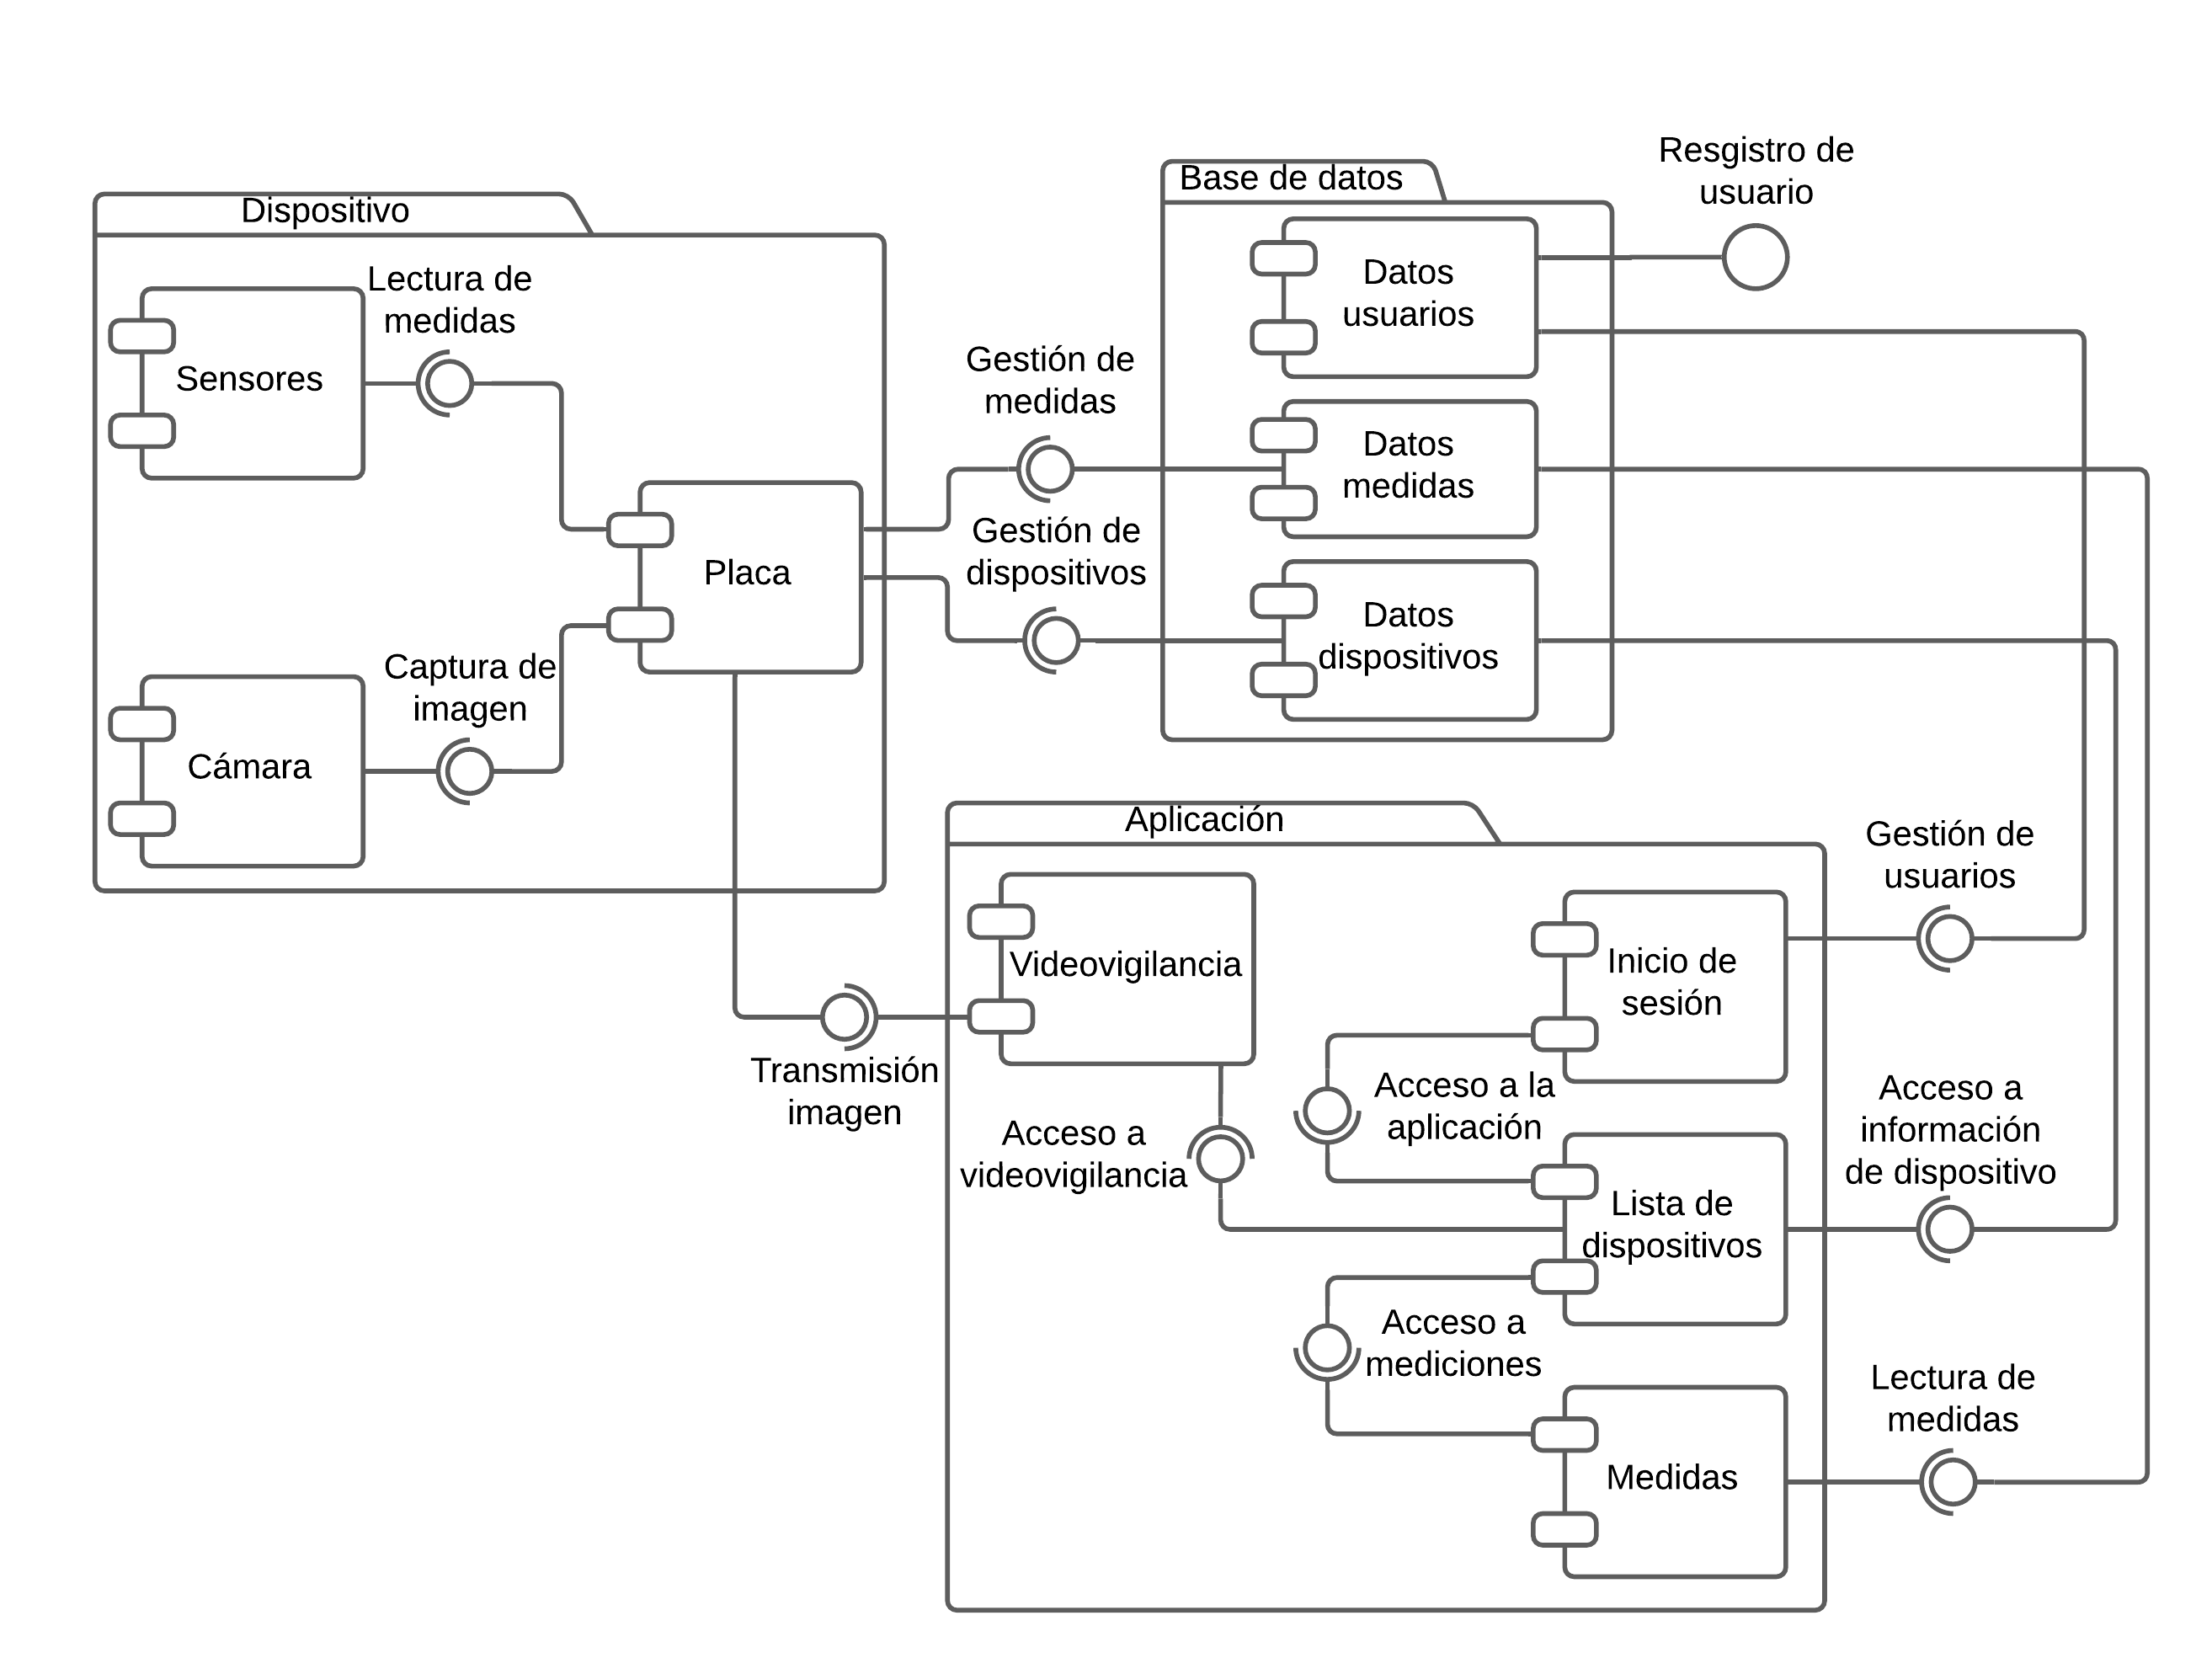
\includegraphics[width=\textwidth]{diagramaComponentes.png}}
\end{figure}
Ahora se procede a explicar los subsistemas y componentes que lo forman:
\begin{itemize}
	\item \textbf{Dispositivo:} Representa a todos los dispositivos que se encuentran conectados al sistema y que toman las medidas del ambiente e imagen del interior de la sala, es por esto por lo que está formado por los siguientes componentes:
	      \begin{itemize}
		      \item \textbf{Sensores:} Cada uno de los componentes conectados al dispositivo que toman medidas del ambiente. Estos están listos para ser empleados y leer las magnitudes correspondientes.
		      \item \textbf{Cámara:} Al igual que los sensores, este es el componente conectado al dispositivo que se encarga de captar imagen del interior de la sala.
		      \item \textbf{Placa:} Componente clave del dispositivo, que dentro del mismo recoge las lecturas de los sensores y la imagen de la sala. Una vez tiene estos datos, se encarga de enviar las mediciones a la base de datos, junto con la información de estado del propio dispositivo. Además, también transmite la imagen de la cámara vía IP para que pueda ser recogida por la aplicación.
	      \end{itemize}
	\item \textbf{Base de datos:} Representa el conjunto de tablas que conforman el modelo de datos, en el que se almacenan las medidas, los datos del dispositivo y las credenciales de los usuarios. Sus componentes son:
	      \begin{itemize}
		      \item \textbf{Datos usuarios:} Es el componente encargado de almacenar las credenciales de usuario, que se usan para acceder a la aplicación. Además, permite que se introduzcan nuevos usuarios mediante su registro.
		      \item \textbf{Datos medidas:} Recibe las medidas de los dispositivos mediante la interfaz gestión de medidas y responde a las solicitudes realizadas por la aplicación.
		      \item \textbf{Datos dispositivos:} Obtiene los datos de estado de los dispositivos que se encuentran en el sistema y da acceso a la aplicación a estos para ser mostrados.
	      \end{itemize}
	\item \textbf{Aplicación:} Es el subsistema con el que interactúa el usuario, al que mediante sus credenciales puede acceder a ver los dispositivos conectados, sus mediciones y la imagen que toman. Está compuesto por:
	      \begin{itemize}
		      \item \textbf{Inicio de sesión:} Es el componente que mediante la comprobación de las credenciales de usuario, permite acceder a la aplicación y estos son verificados mediante la base de datos.
		      \item \textbf{Lista de dispositivos:} Una vez se ha iniciado sesión en la aplicación, este permite ver los dispositivos conectados y su estado, que se obtiene de la base de datos.
		      \item \textbf{Medidas:} Es el encargado de mostrar de manera gráfica y tabular las diferentes medidas tomadas por el dispositivo de la lista de dispositivos, estas medidas se extraen de la base de datos.
		      \item \textbf{Videovigilancia:} Es el componente encargado de mostrar la imagen en tiempo real del dispositivo instalado en la sala, recibe la imagen mediante la retransmisión del dispositivo y es accesible mediante la lista de dispositivos.
	      \end{itemize}
\end{itemize}

En las siguientes secciones se define la parte de Modelo (\autoref{sec:modelo}), Vista (\autoref{sec:interfaz}) y Controlador (\autoref{sec:servidor} y \autoref{sec:hardware}).
1\pagebreak

\section{Modelo de datos}\label{sec:modelo}
En este proyecto la base de datos es uno de los elementos más importantes que componen el sistema, no solo para permitir el acceso del personal autorizado a la aplicación, sino porque almacena el histórico de las medidas tomadas en la sala, lo que en un futuro permitirá analizar cuál ha sido el estado de esta.

La base de datos está alojada en el servidor, donde la aplicación puede acceder a ella más fácilmente para su visualización y consulta. Además, facilita que se puedan centralizar las medidas en un único lugar, para el caso en el que se tuvieran múltiples dispositivos en un edificio y se deseara consultarlos desde un mismo punto.

Como se comentó en la \autoref{subsec:servidorDB} se utiliza una base de datos MariaDB, que se administra mediante phpMyAdmin~\cite{phpmyadmin_phpmyadmin_nodate}, que es un administrador de base de datos para realizar la mayoría de las tareas de una manera más sencilla y eficiente.

\subsection{Estructura de tablas de la base de datos}\label{subsec:estructura-de-tablas-de-la-base-de-datos}
Se presentan en esta subsección las tablas que componen la base de datos, indicando la utilidad de cada una de ellas y los datos, con sus tipos, que se almacenan en ellas. Antes de pasar a explicarlas en más detalle en la \autoref{fig:distDB} se puede ver un resumen de estas.
\begin{figure}[H]
	\ffigbox[\FBwidth]
	{\caption{Distribución de tablas en la base de datos}
		\label{fig:distDB}}
	{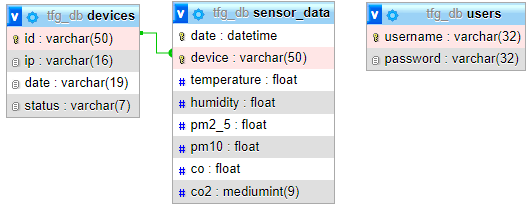
\includegraphics[scale=0.85]{db_dist.png}}
\end{figure}
\subsubsection{Tabla de usuarios}
En esta tabla se almacenan las credenciales de los usuarios que utilicen la aplicación. Estas credenciales se consultan cuando un usuario trata de iniciar sesión y son añadidas por el administrador del sistema en esta tabla. Es importante destacar que la contraseña se almacena en formato hash (encriptada) para evitar que se pueda leer si llega a haber alguna intrusión. 
\pagebreak

A continuación, en la \autoref{tab:tabla_users} se muestra la estructura de la tabla:
\begin{table}[H]
	\centering
	\caption{Tabla users BBDD}
	\label{tab:tabla_users}
	\resizebox{\textwidth}{!}{%
		\begin{tabular}{|p{.2\textwidth}|p{.2\textwidth}|p{.6\textwidth}|}
			\hline
			\rowcolor[HTML]{BFBFBF}
			\multicolumn{1}{|c|}{\cellcolor[HTML]{BFBFBF}{\color[HTML]{000000} \textbf{Nombre}}} & \multicolumn{1}{c|}{\cellcolor[HTML]{BFBFBF}{\color[HTML]{000000} \textbf{Tipo}}} & \multicolumn{1}{c|}{\cellcolor[HTML]{BFBFBF}{\color[HTML]{000000} \textbf{Descripción}}} \\ \hline
			username                                                                             & varchar(32)                                                                       & Nombre de usuario que identifica unívocamente al usuario                                 \\ \hline
			password                                                                             & varchar(32)                                                                       & MD5 de la clave de acceso que debe proporcionar para verificar su identidad              \\ \hline
		\end{tabular}%
	}
\end{table}
La clave primaria es el username, de esta manera no hay ningún problema de duplicidad de usuarios en la base de datos.

\subsubsection{Tabla de dispositivos}
En esta tabla se registran los dispositivos que se han conectado con el servidor, estos dispositivos son los que se pueden consultar desde la aplicación y que se muestran con la fecha de actualización junto con su estado actual.

En la \autoref{tab:tabla_devices} se pueden ver los atributos que la componen:

\begin{table}[H]
	\centering
	\caption{Tabla devices BBDD}
	\label{tab:tabla_devices}
	\resizebox{\textwidth}{!}{%
		\begin{tabular}{|p{.2\textwidth}|p{.2\textwidth}|p{.6\textwidth}|}
			\hline
			\rowcolor[HTML]{BFBFBF}
			\multicolumn{1}{|c|}{\cellcolor[HTML]{BFBFBF}{\color[HTML]{000000} \textbf{Nombre}}} & \multicolumn{1}{c|}{\cellcolor[HTML]{BFBFBF}{\color[HTML]{000000} \textbf{Tipo}}} & \multicolumn{1}{c|}{\cellcolor[HTML]{BFBFBF}{\color[HTML]{000000} \textbf{Descripción}}} \\ \hline
			id                                                                                   & varchar(50)                                                                       & Nombre identificativo del dispositivo, su dirección física                               \\ \hline
			ip                                                                                   & varchar(16)                                                                       & IP de la red local desde la que se puede acceder a sus datos                             \\ \hline
			date                                                                                 & datetime                                                                          & Fecha de la última actualización de estado                                               \\ \hline
			status                                                                               & varchar(7)                                                                        & Estado del dispositivo, Online u Offline                                                 \\ \hline
		\end{tabular}%
	}
\end{table}
Como en la \autoref{tab:tabla_users} la clave primaria de esta es un nombre representativo, en este caso el id, que identifica inequívocamente al dispositivo, de esta manera se puede utilizar para consultar los datos de un dispositivo en concreto. Cuando sea necesario, se puede variar la IP a la que está conectado, la fecha y el estado, pero el nombre identificador no se puede cambiar.

\subsubsection{Tabla de medidas}
Es la tabla más importante como ya se ha mencionado. En esta tabla se guardan las mediciones que han tomado todos los dispositivos conectados. Estos datos son los que se muestran en la página del dispositivo dentro de la aplicación, junto con su imagen en tiempo real. Las medidas que se almacenan son: temperatura, humedad, PM$_{2,5}$, PM$_{10}$, CO y CO$_2$.

Los datos que la componen se exponen en la \autoref{tab:tabla_sensor_data}:

\begin{table}[H]
	\centering
	\caption{Tabla sensor\_data BBDD}
	\label{tab:tabla_sensor_data}
	\resizebox{\textwidth}{!}{%
		\begin{tabular}{|p{.2\textwidth}|p{.2\textwidth}|p{.6\textwidth}|}
			\hline
			\rowcolor[HTML]{BFBFBF}
			\multicolumn{1}{|c|}{\cellcolor[HTML]{BFBFBF}{\color[HTML]{000000} \textbf{Nombre}}} & \multicolumn{1}{c|}{\cellcolor[HTML]{BFBFBF}{\color[HTML]{000000} \textbf{Tipo}}} & \multicolumn{1}{c|}{\cellcolor[HTML]{BFBFBF}{\color[HTML]{000000} \textbf{Descripción}}} \\ \hline
			date                                                                                 & datetime                                                                          & Fecha en la que se ha tomado la medida                                                   \\ \hline
			device                                                                               & varchar(50)                                                                       & Identificador del dispositivo que captó la medida                                        \\ \hline
			temperature                                                                          & float                                                                             & Temperatura de la sala                                                                   \\ \hline
			humidity                                                                             & float                                                                             & Humedad de la sala                                                                       \\ \hline
			pm2\_5                                                                               & float                                                                             & Cantidad de partículas de 2,5 $\mu m$ en la sala                                         \\ \hline
			pm10                                                                                 & float                                                                             & Cantidad de partículas de 10 $\mu m$ en la sala                                          \\ \hline
			co                                                                                   & float                                                                             & Porcentaje de CO en el aire de la sala                                                   \\ \hline
			co2                                                                                  & mediumint(9)                                                                      & Partículas por millón de CO$_2$ en la sala                                               \\ \hline
		\end{tabular}%
	}
\end{table}
Las claves primarias son date y device, estas claves identifican de manera única a cada una de las medidas, por lo que se puede consultar una medida concreta de un dispositivo específico.

Además, existe una relación directa con la tabla devices en cuanto a que el campo device es una clave ajena del campo id, de esta manera cuando un dispositivo sea eliminado o actualizado se propaga a esta tabla.

\section{Interfaz de Usuario}\label{sec:interfaz}
En esta sección se trata otro de los elementos clave del sistema, la interfaz de usuario. Esta hace posible el uso del sistema a personas no expertas, de manera que puedan manipularlo y hacer uso de este sin la necesidad de saber cómo se desarrolla un sistema de estas características.

La parte del sistema a la que se ha dotado de interfaz es la responsable de mostrar las medidas y video de las salas, tal y como ha solicitado el cliente. Para lograr esto se utiliza una página web, que se ha diseñado en HTML y CSS, con la que se puede acceder a toda esta información de una manera sencilla y visual. En cuanto a la lógica para obtener la información y moverse por las pantallas, se emplea PHP\@.

La web, además, es \textit{responsive} por lo que es totalmente funcional tanto en dispositivos de altas resoluciones (televisiones, ordenadores de sobremesa, portátiles, etc.), como en dispositivos de bajas resoluciones (móviles, tablets, etc.).

En la \autoref{fig:flujo_interfaz} se muestra el flujo de pantallas e interacciones que se sigue al acceder a la aplicación web, más tarde se explica en detalle cada una de las pantallas de la interfaz y que interacciones permite.
\begin{figure}[H]
	\ffigbox[\FBwidth]
	{\caption{Diagrama de flujo de la web}
		\label{fig:flujo_interfaz}}
	{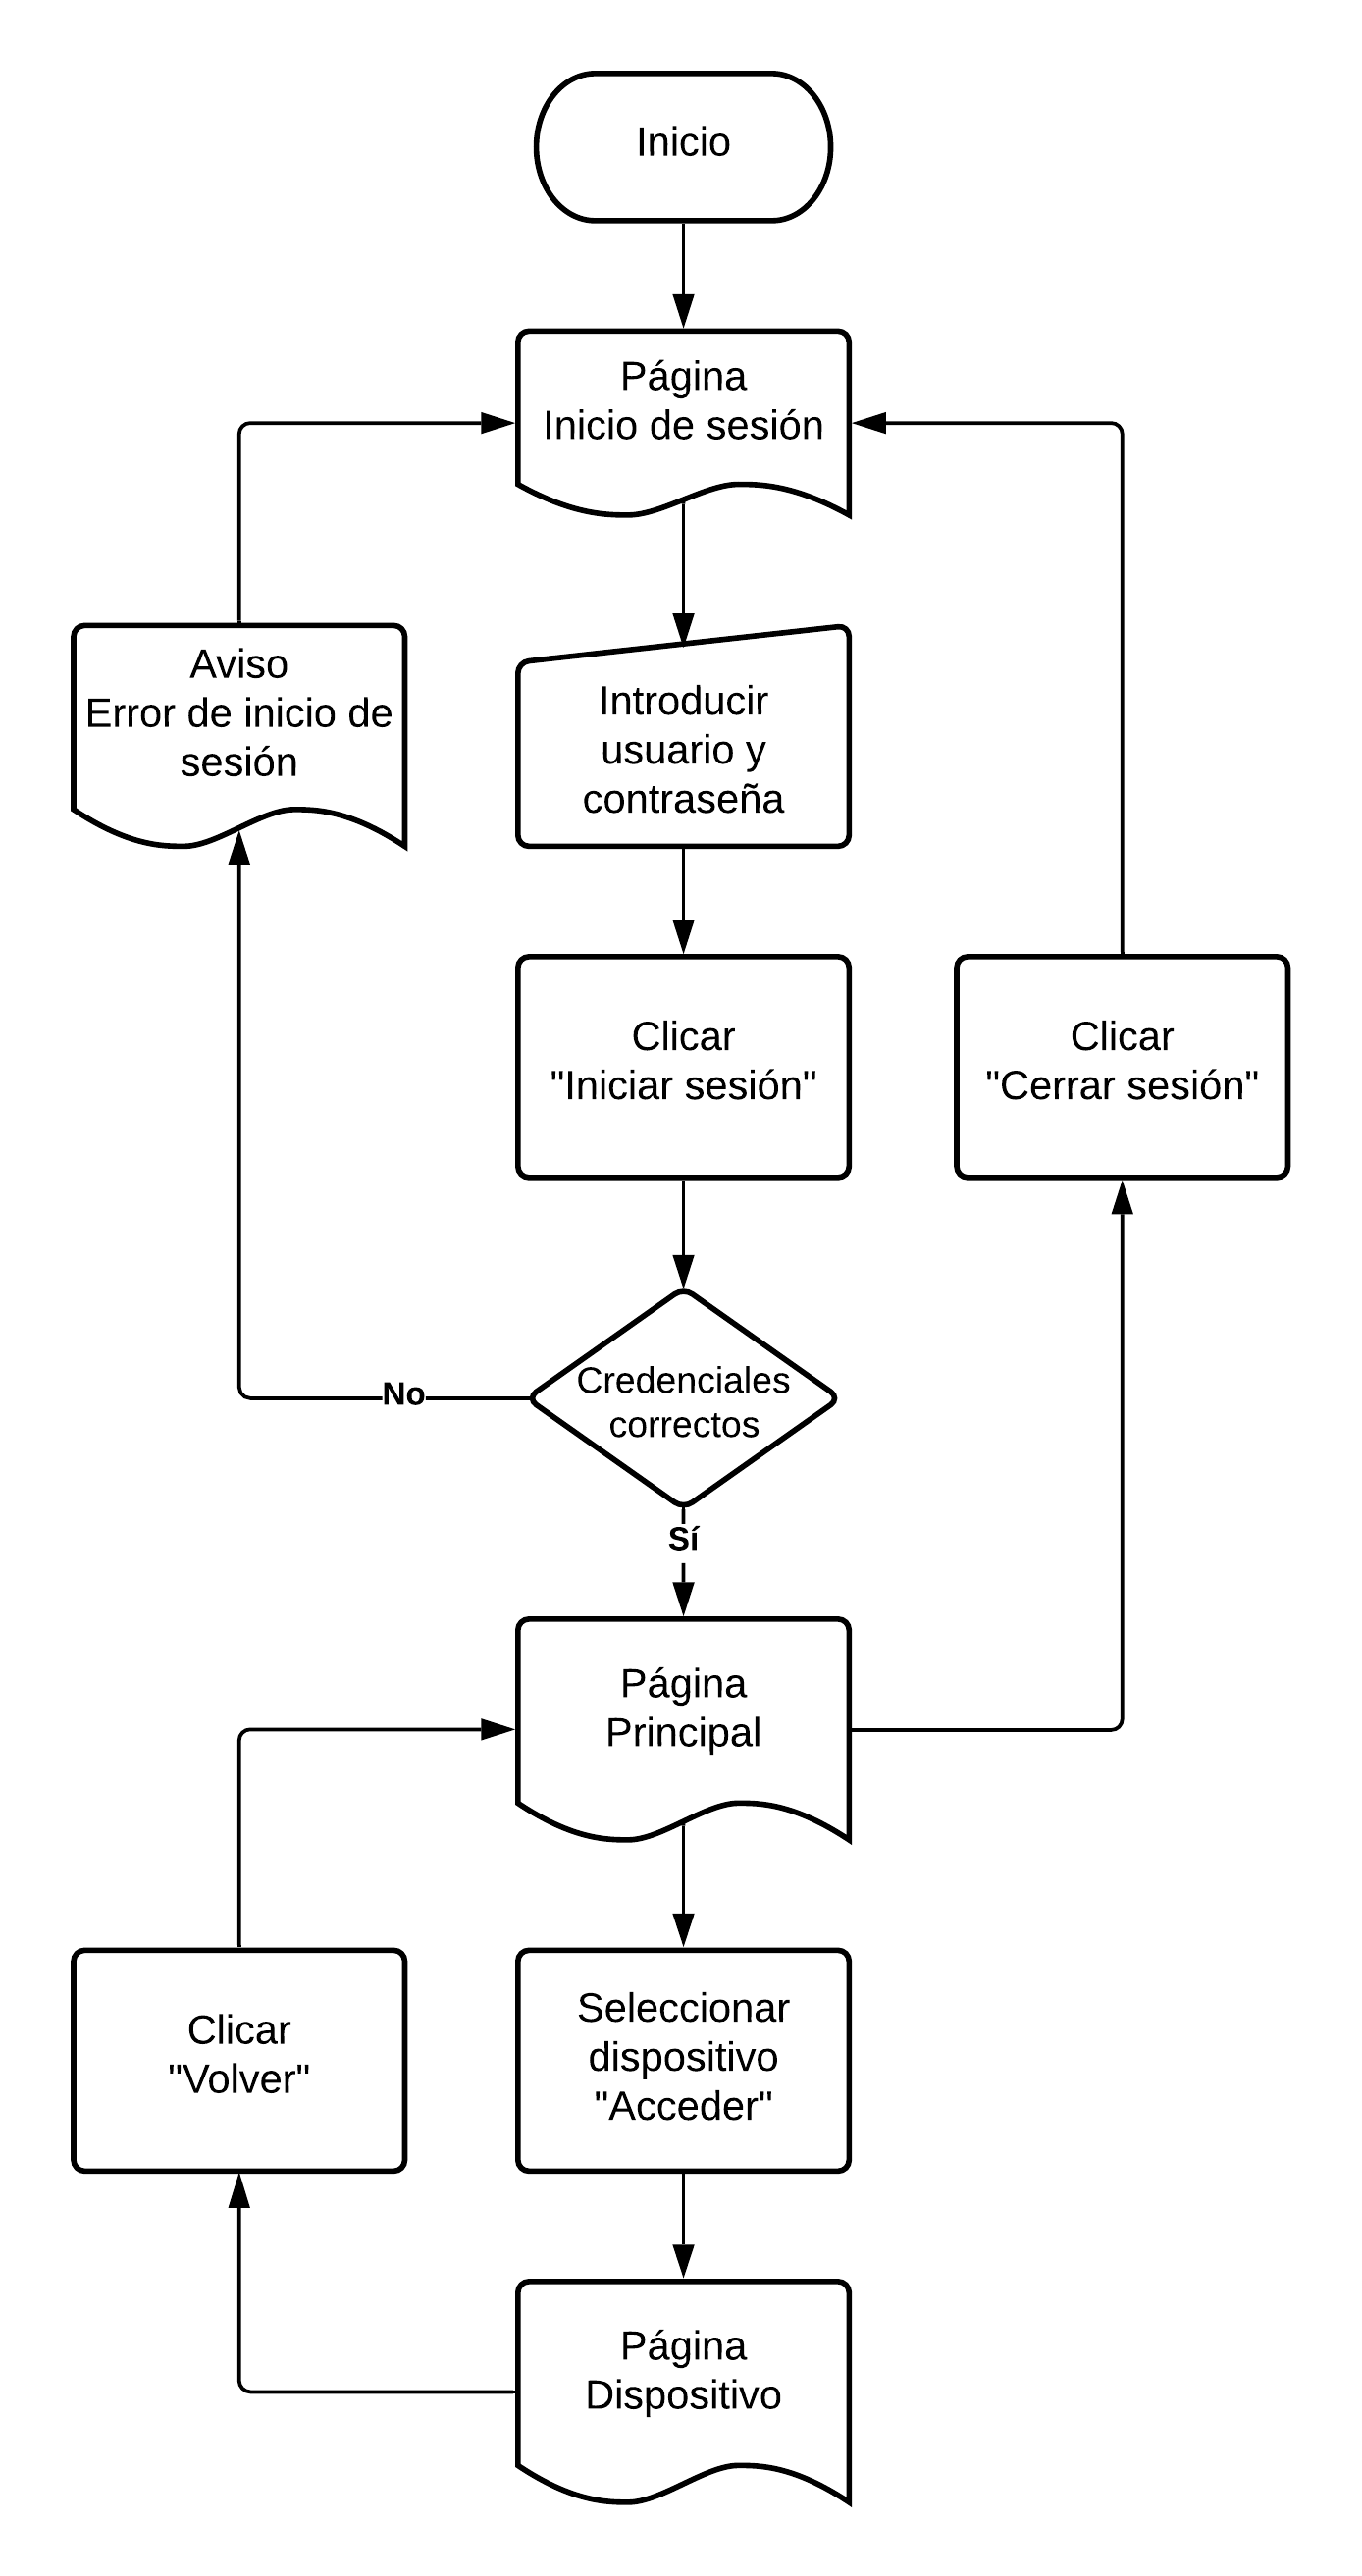
\includegraphics[scale=1]{flujoInterfaz.png}}
\end{figure}

\subsection{Página: Inicio de sesión}\label{subsec:iLogin}
Es la primera pantalla que se encuentra el usuario cuando accede a la aplicación, en esta, como se puede ver en la \autoref{fig:iLogin} se le solicita introducir su nombre de usuario y contraseña de acceso. Esta pantalla es fundamental para garantizar la seguridad del centro, de manera que no accedan personas no autorizadas y que puedan poner en riesgo su seguridad.
\begin{figure}[H]
	\ffigbox[\textwidth]
	{\caption{Interfaz de inicio de sesión}
		\label{fig:iLogin}}
	{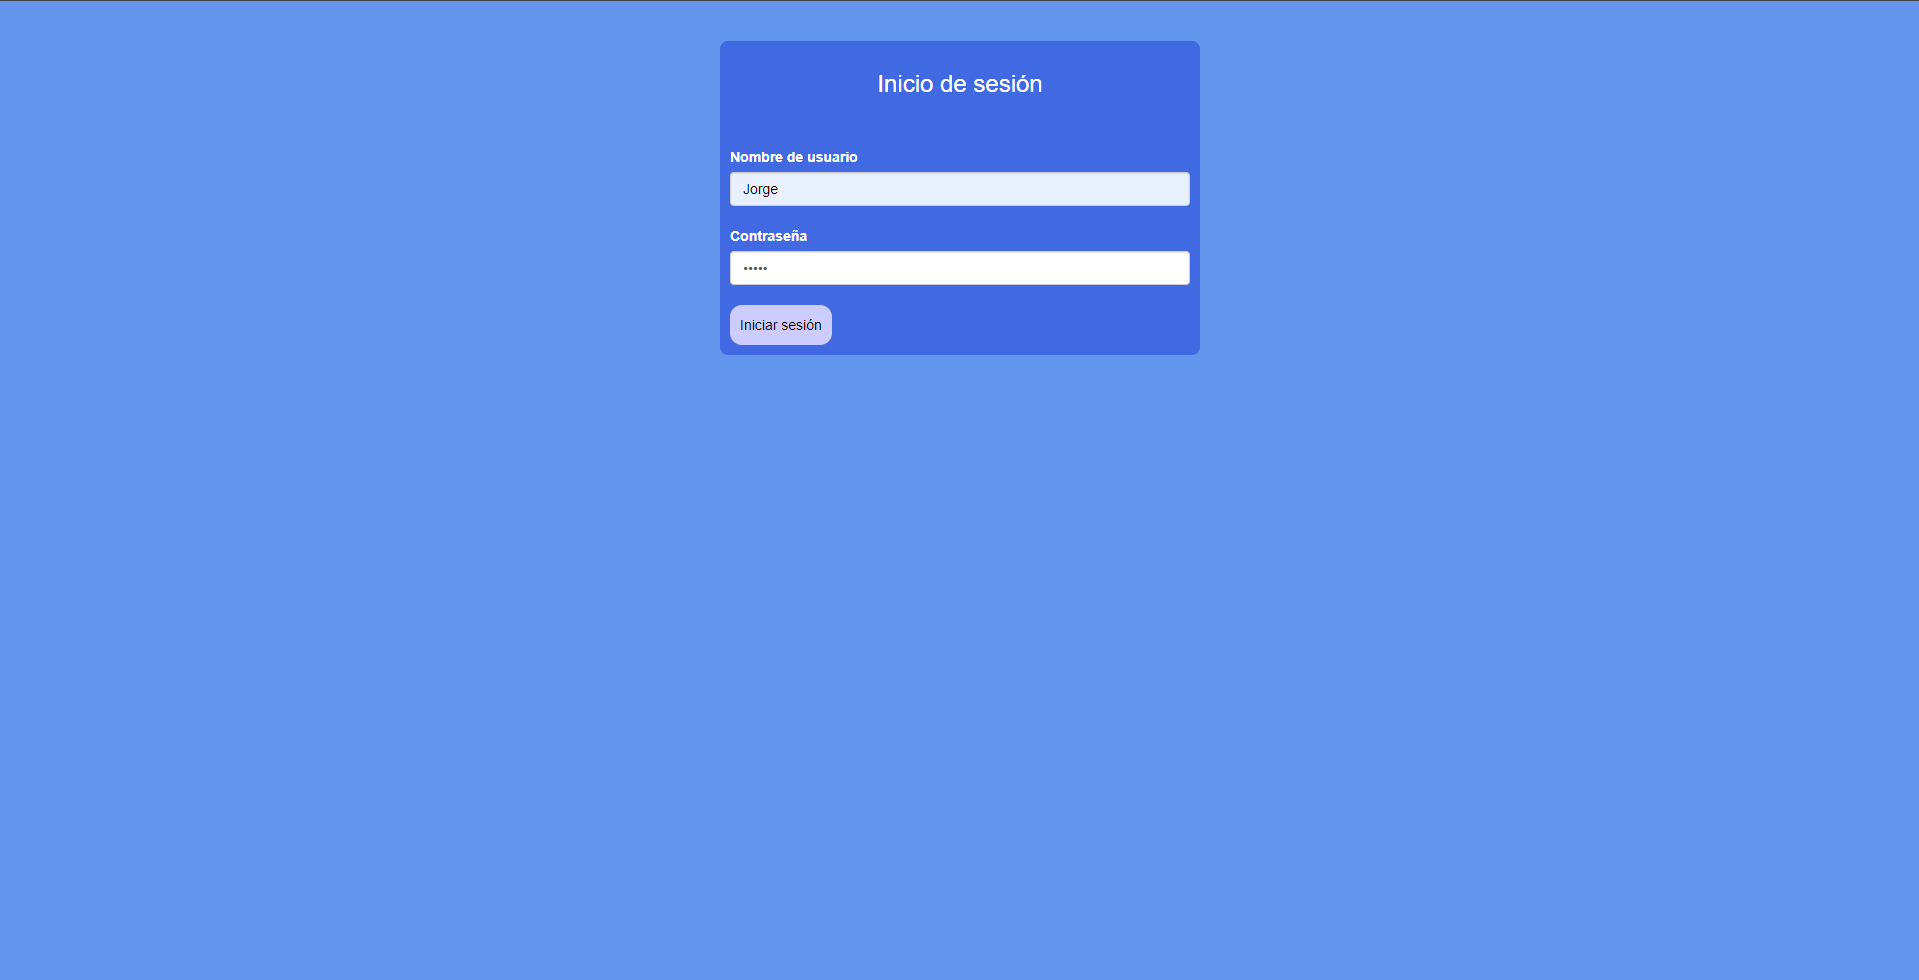
\includegraphics[width=\textwidth]{login.png}}
\end{figure}
Como se puede observar, la paleta de colores se adapta a lo solicitado por el cliente, utilizando colores de la gama de los azules que contrasten entre ellos, de manera que se puedan visualizar sin dificultad todos los elementos de esta. Los códigos RGB hexadecimales elegidos son:
\begin{itemize}
	\item Primario: \#4169e1
	\item Secundario: \#4169e1
	\item Primario claro: \#191970
	\item Secundario Oscuro: \#ccccff
	\item Resaltado: \#9e9eff
	\item Gris: \#dddddd
\end{itemize}
En el primer campo, correspondiente al nombre de usuario, se muestra el texto escrito, sin embargo, en el de la contraseña los caracteres del texto se sustituye visualmente por asteriscos, garantizando la privacidad de la contraseña.

En el caso de introducir unas credenciales no registradas en el sistema se avisa al usuario de que revise lo que ha escrito, "<Compruebe las credenciales">, dado que si no coinciden no se puede garantizar su identidad.

Por otro lado, también se deben completar ambos campos, si esto no es así se lanza un aviso al usuario informándole de que los debe cumplimentar si desea acceder, "<Ambos campos son obligatorios">.

Una vez el usuario ha completado los campos puede hacer clic en el botón "<Iniciar sesión"> y si cumple todo lo anterior le lleva a la pantalla principal descrita en la \autoref{subsec:iPrincipal}.

En cuanto a la versión móvil, se ha ajustado el tamaño del formulario para que se adapte y sea legible incluso en resoluciones pequeñas. Además, el tamaño de letra es suficientemente grande, 14 píxeles para formulario y 10 píxeles para el botón, como para que se pueda leer correctamente tanto en grandes como en pequeñas resoluciones.
\begin{figure}[H]
	\ffigbox[\FBwidth]
	{\caption{Interfaz de inicio de sesión en móvil}
		\label{fig:iLoginM}}
	{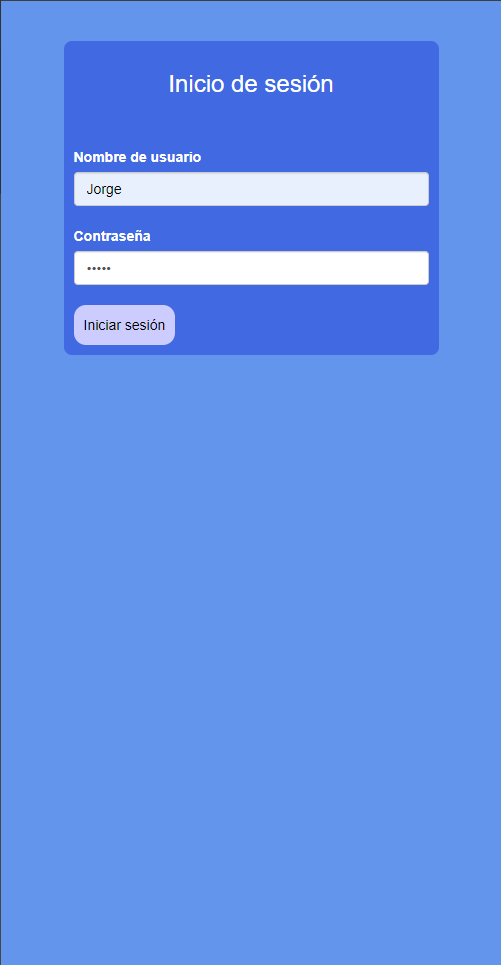
\includegraphics[scale=0.55]{loginM.png}}
\end{figure}

\subsection{Página: Principal}\label{subsec:iPrincipal}
Una vez el usuario ha iniciado la sesión de manera satisfactoria, se pasa a la pantalla mostrada en la \autoref{fig:iPrincipal}, en la que se puede ver, que muestra un mensaje de saludo, indicando el nombre de usuario.

La clave de esta pantalla es la lista de los dispositivos, en la que se muestran de manera tabular los datos de estos. Se imprime, para cada dispositivo, los datos almacenados en la base.
\vspace{.5cm}
\begin{figure}[H]
	\ffigbox[\textwidth]
	{\caption{Interfaz de pantalla principal}
		\label{fig:iPrincipal}}
	{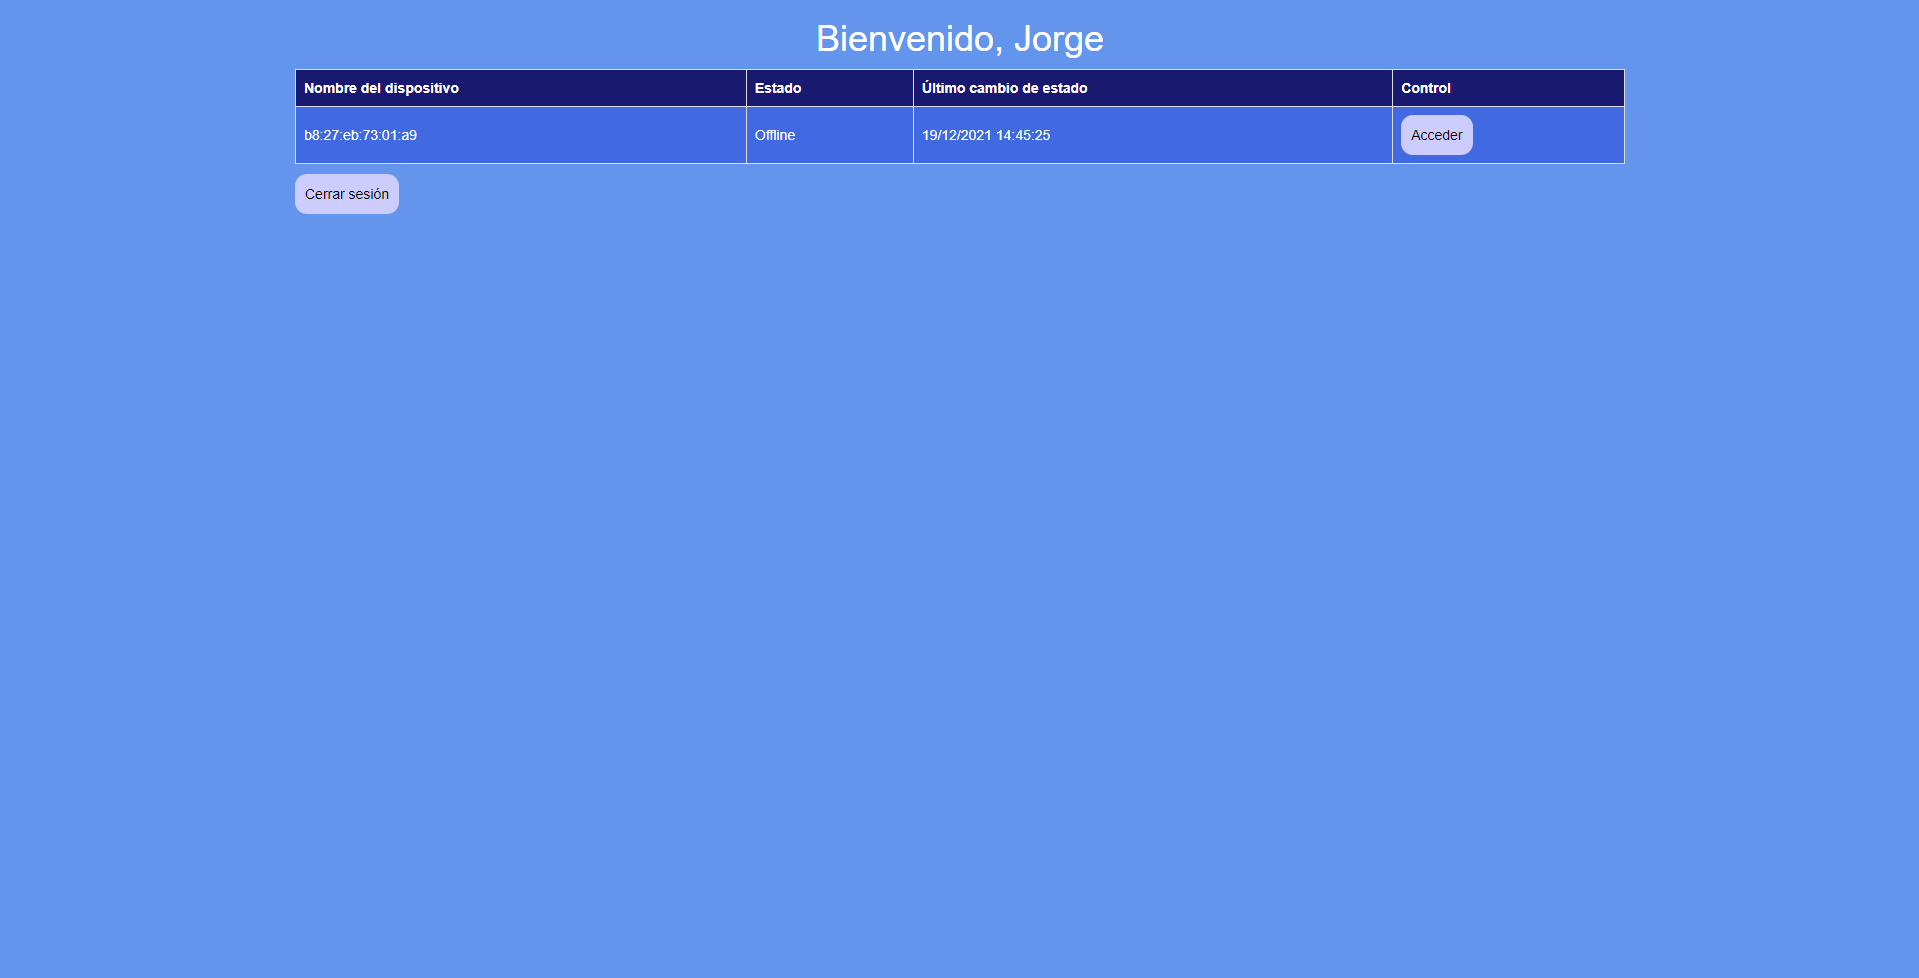
\includegraphics[width=\textwidth]{devices.png}}
\end{figure}
En la última posición de cada fila de dispositivos hay un botón en el que pone "<Acceso"> que redirige a la página de dispositivo, que se describe en la \autoref{subsec:iDispositivo}.

En la parte inferior aparece un botón con el texto "<Cerrar sesión"> que como su propio nombre indica, cierra la sesión y devuelve a la página de inicio de sesión, \autoref{subsec:iLogin}.

Por último, en la versión móvil la tabla pasa a ocupar el ancho completo de la pantalla para que se pueda ver claramente el botón de la última posición y facilitar acceder al dispositivo. En cuanto al texto de saludo, se ha decidido mantenerlo, pero ajustándose para que no se salga de la pantalla, evitando el \textit{scroll} lateral.
\vspace{.5cm}
\begin{figure}[H]
	\ffigbox[\FBwidth]
	{\caption{Interfaz de pantalla principal en móvil}
		\label{fig:iPrincipalM}}
	{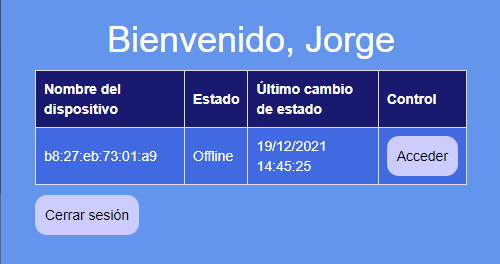
\includegraphics[scale=0.6]{devicesM.png}}
\end{figure}

\subsection{Página: Dispositivo}\label{subsec:iDispositivo}
Esta pantalla muestra la información clave de este proyecto, la imagen de la cámara del dispositivo y las medidas tomadas. 

A esta pantalla se accede una vez se ha seleccionado un dispositivo en la página principal, \autoref{subsec:iPrincipal}, y tiene la apariencia que se muestra en la \autoref{fig:iDispositivoI}, \autoref{fig:iDispositivoII} y \autoref{fig:iDispositivoIII}.

En primer lugar, en la parte superior se muestra el nombre que identifica al dispositivo, de manera que se pueda saber, en todo momento, que datos se están consultando.

Inmediatamente después, se muestra un cuadro con la imagen en tiempo real de la cámara del dispositivo.
\begin{figure}[H]
	\ffigbox[\textwidth]
	{\caption{Interfaz de dispositivo I}
		\label{fig:iDispositivoI}}
	{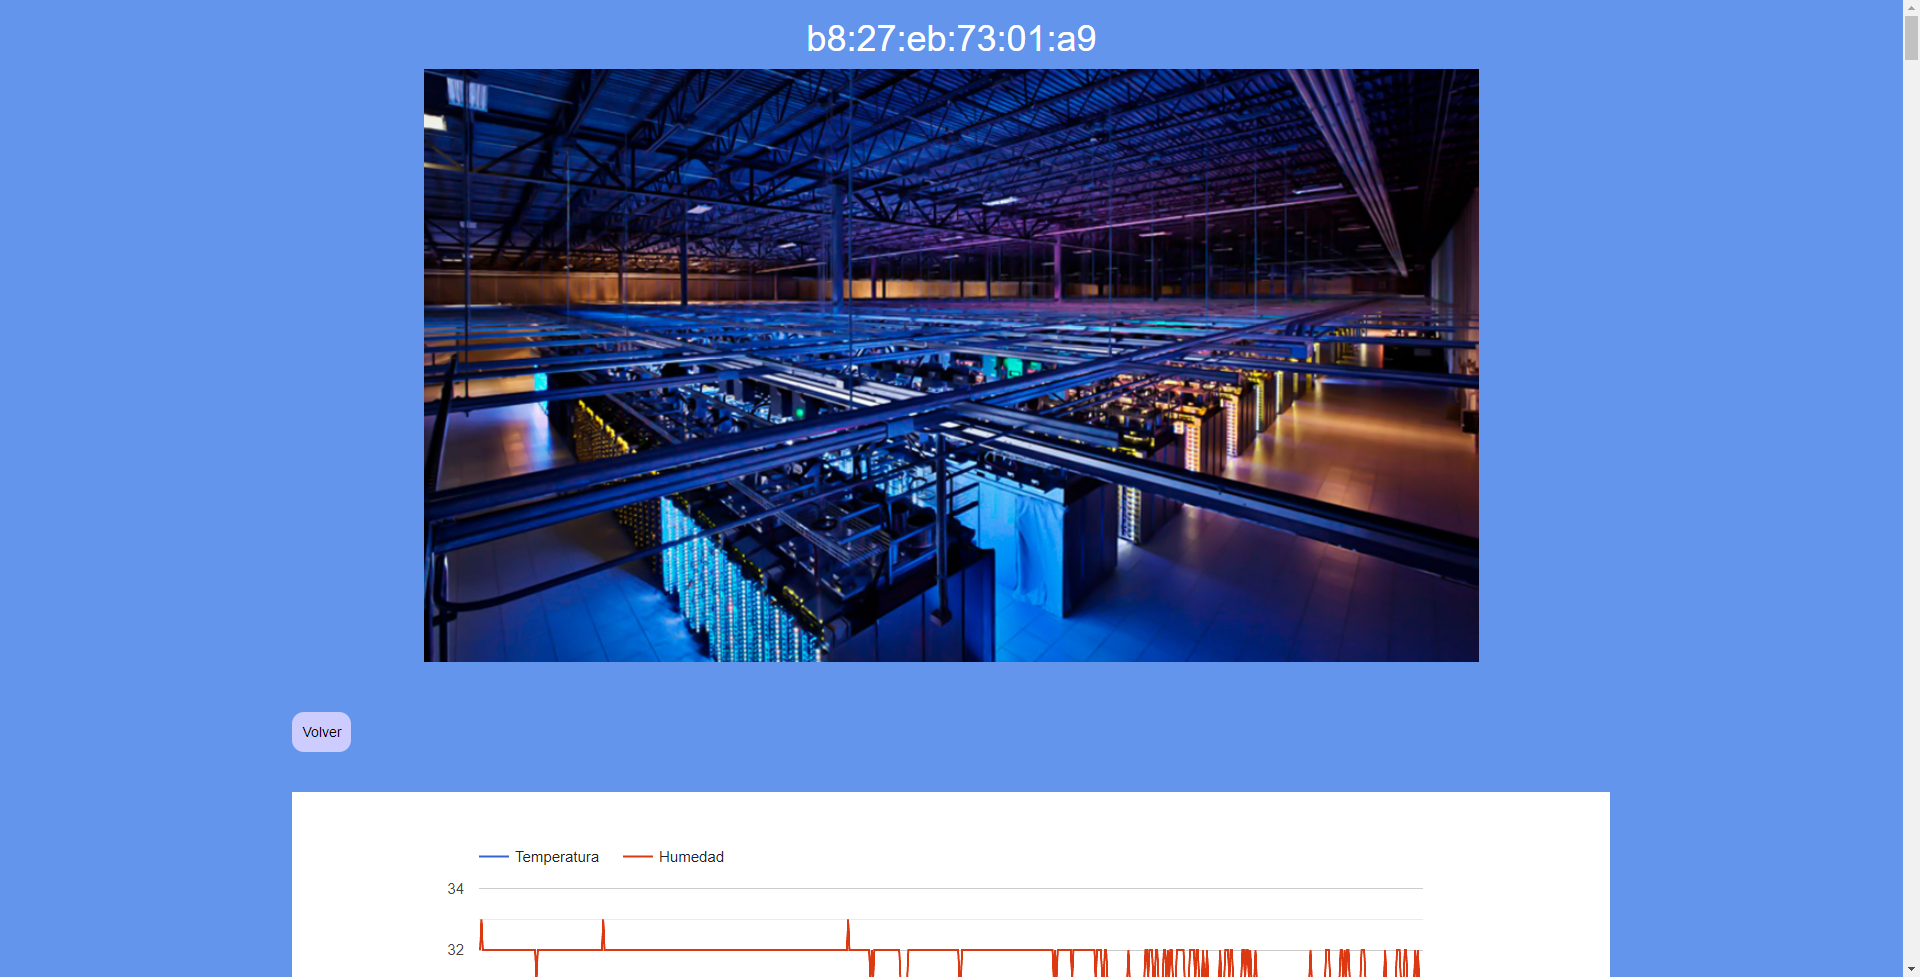
\includegraphics[width=\textwidth]{medidas1.png}}
\end{figure}
A continuación, se muestran todas las medidas, primero de manera gráfica y después de manera tabular.

La parte visual de las medidas se divide en 3 gráficas distintas, para poder ver mejor como progresan en el tiempo sin que haya problemas de escalas entre ellas y sin saturar la pantalla. Las gráficas son:
\begin{itemize}
	\item Temperatura y Humedad.
	\item PM$_{2,5}$, PM$_{10}$ y CO\@.
	\item CO$_2$.
\end{itemize}
\begin{figure}[H]
	\ffigbox[\textwidth]
	{\caption{Interfaz de dispositivo II}
		\label{fig:iDispositivoII}}
	{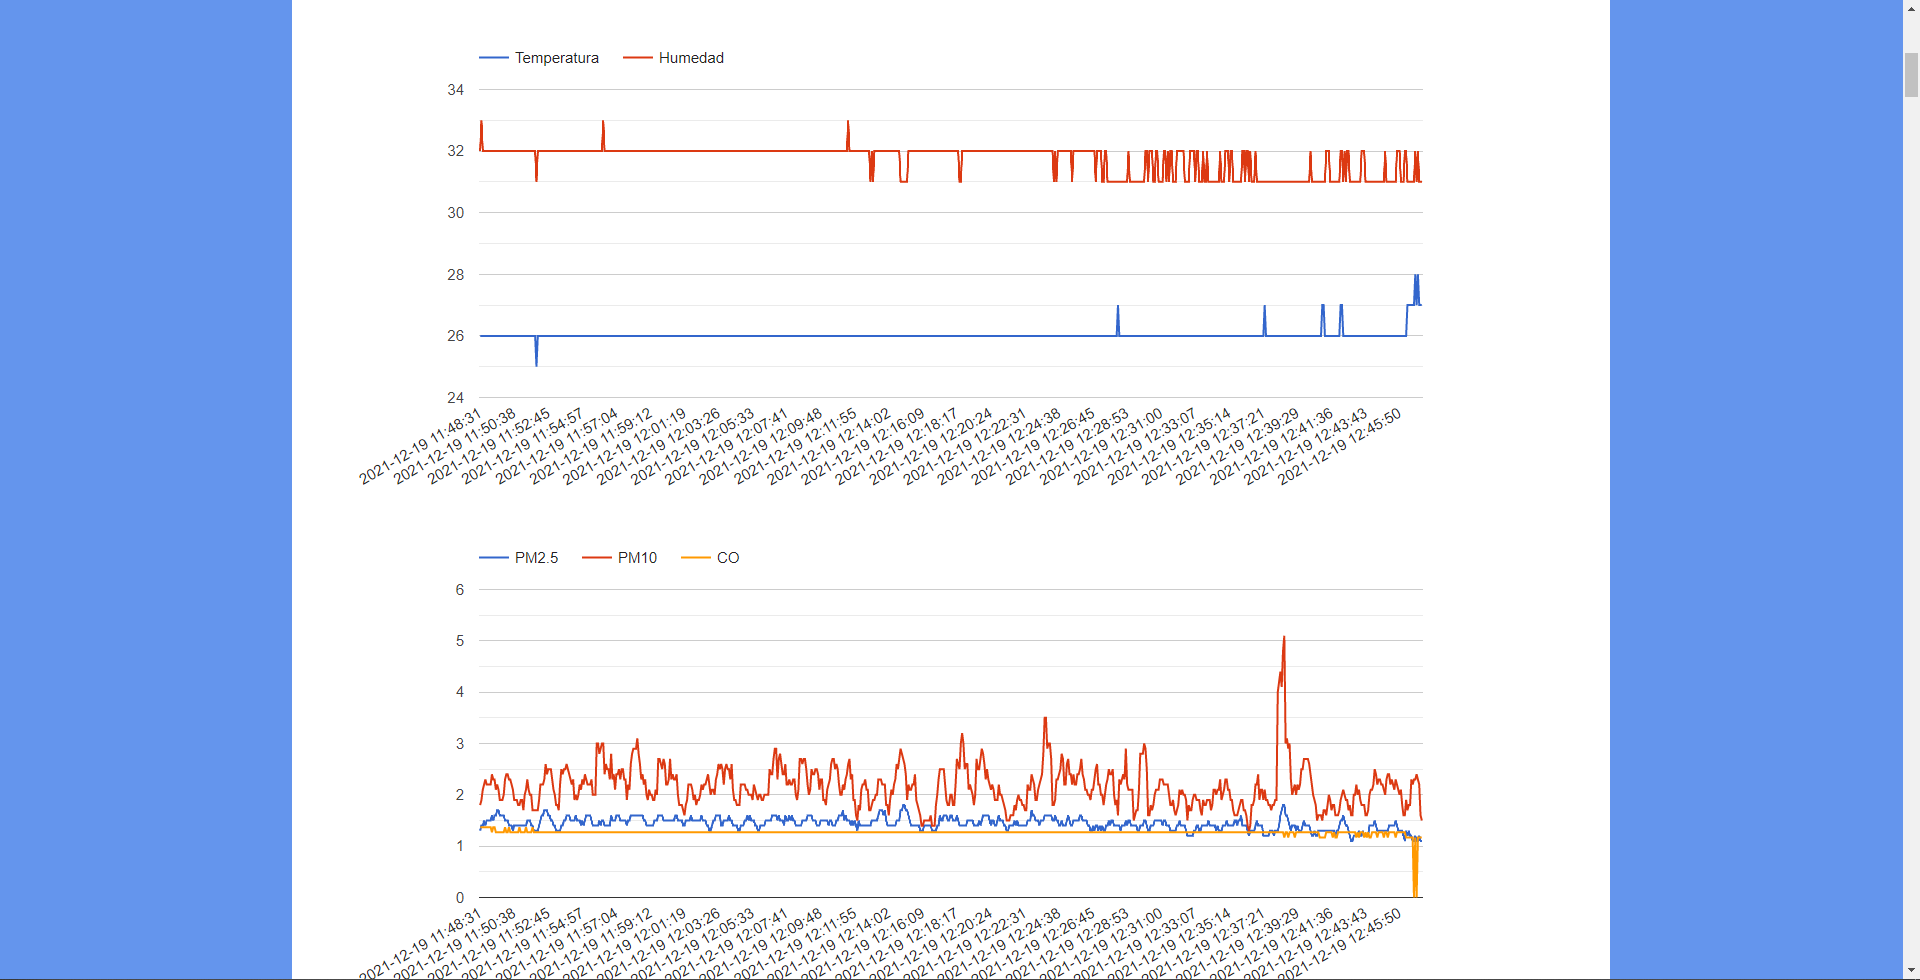
\includegraphics[width=\textwidth]{medidas2.png}}
\end{figure}
En cuanto a la forma tabular, mediante una tabla se muestran las medidas de manera cronológica, de más reciente a más antigua. Esta tabla está compuesta por los 720 últimos registros, que cubren la última hora de mediciones de la sala, puesto que se toma una medida cada 5 segundos.
\vspace{.5cm}
\begin{figure}[H]
	\ffigbox[\textwidth]
	{\caption{Interfaz de dispositivo III}
		\label{fig:iDispositivoIII}}
	{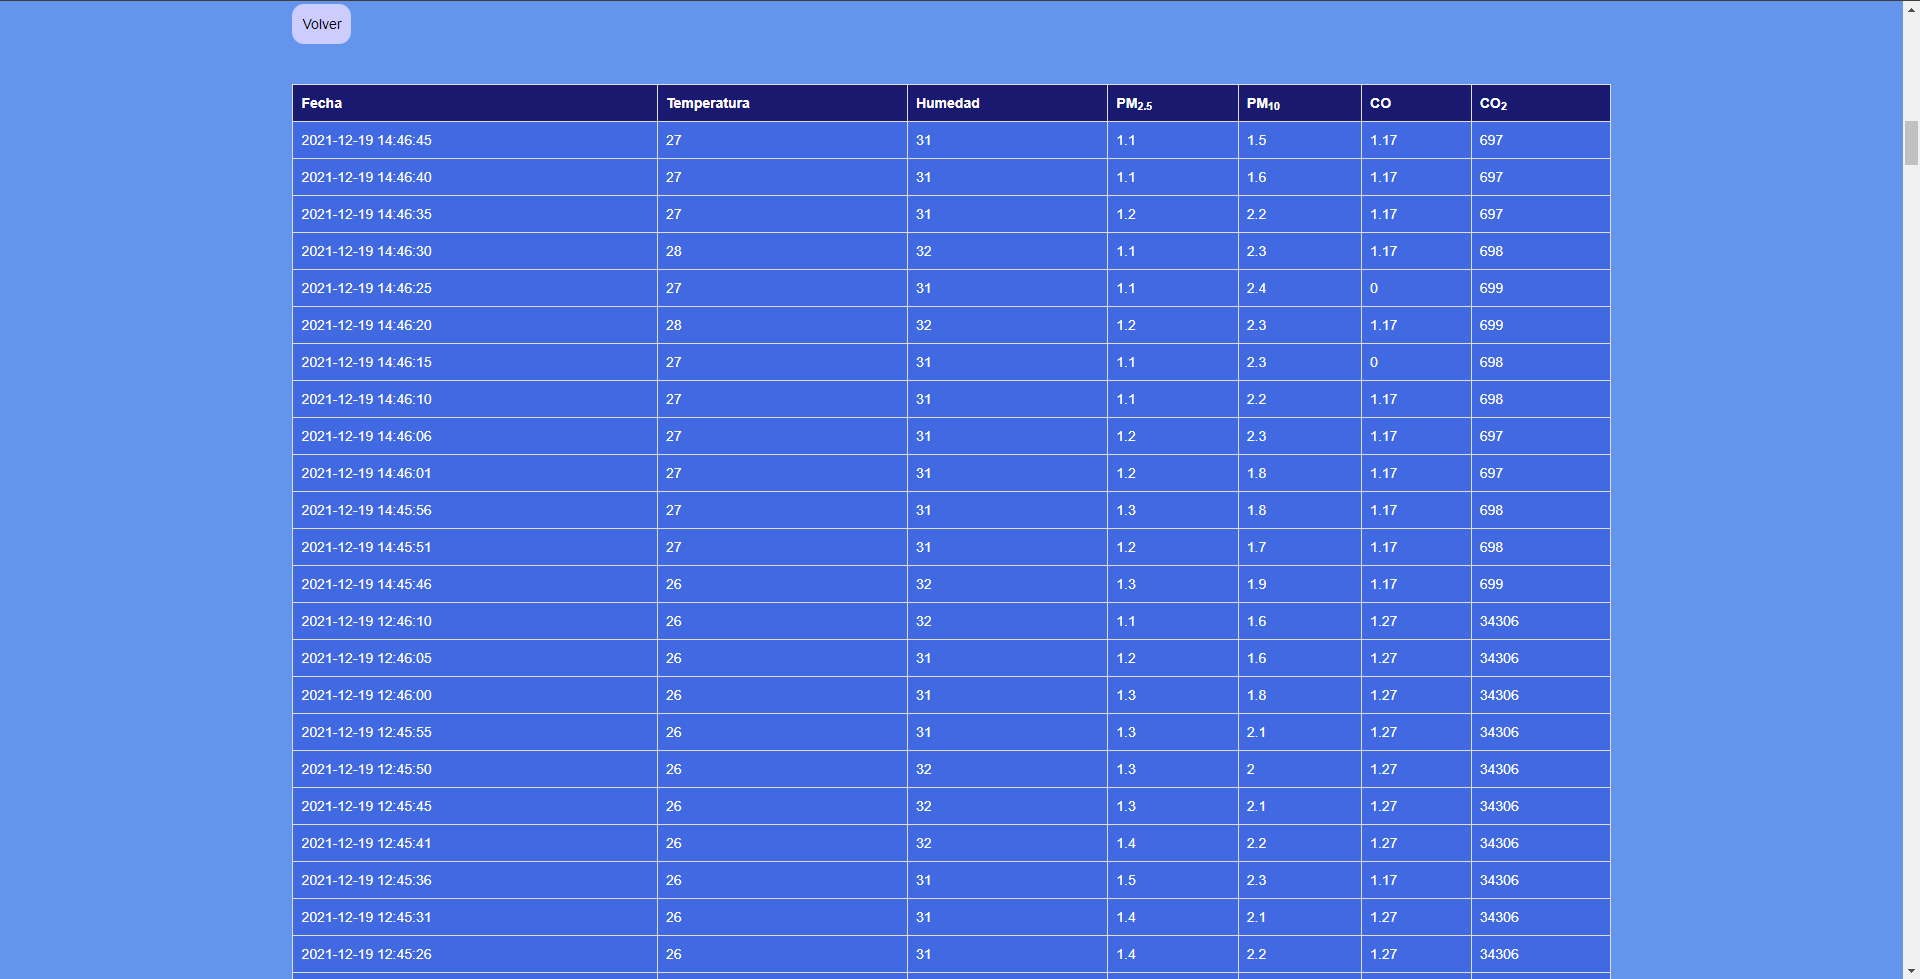
\includegraphics[width=\textwidth]{medidas3.png}}
\end{figure}

Para la versión móvil se ajusta el tamaño de la cámara, gráficas y tabla al ancho del dispositivo, de manera que se puedan visualizar bien todos los datos, evitando así tener que hacer zum en la pantalla.
\pagebreak

Además, las gráficas ofrecen la posibilidad de acceder a un dato en particular si se hace clic o toca una sección específica, indicando los valores y momento específicos.
\begin{figure}[H]
	\ffigbox[\FBwidth]
	{\caption{Interfaz de dispositivo en móvil}
		\label{fig:iDispositivoMI}}
	{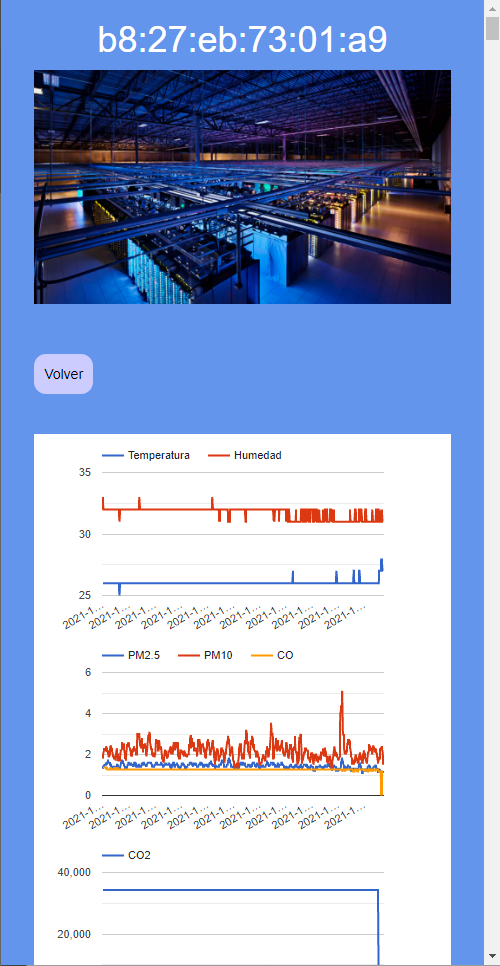
\includegraphics[scale=0.5]{medidas1M.png}
		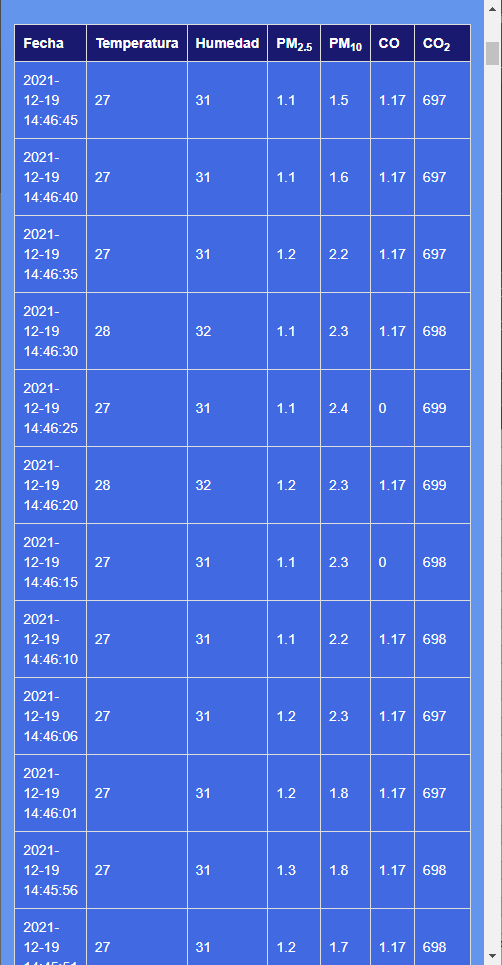
\includegraphics[scale=0.5]{medidas3M.png}}
\end{figure}

\section{Servidor}\label{sec:servidor}
Como ya se especifica en la \autoref{subsec:servidorDB}, el servidor que se emplea para alojar la página web es Apache, que cubre todas las necesidades de la aplicación, dado que permite lanzar al público un sitio web desarrollado en el lenguaje PHP. Este lenguaje de desarrollo web facilita la implementación de la lógica y acceso a la base de datos, a la vez que diseñar las pantallas vistas en la \autoref{sec:interfaz}. 

En el mismo servidor se aloja la base de datos tal y como ha quedado descrita en la \autoref{sec:modelo}, eso permite que sea accesible para el dispositivo de medición y videovigilancia, que posee los permisos para acceder a la misma.
\pagebreak

\section{Hardware}\label{sec:hardware}
En cuanto a la parte física del proyecto, se detalla en esta sección cuáles son las conexiones entre los diferentes elementos que se describieron en la \autoref{sec:hardwareSoftware} y que son los elegidos para formar parte de este. La conexión se resume en el esquema de la \autoref{fig:circuito}. Este esquema se ha realizado con Fritzing~\cite{fritzing_fritzing_nodate} que permite de una manera sencilla importar y conectar los componentes.
\begin{figure}[H]
	\ffigbox[\textwidth]
	{\caption{Esquema de conexiones dispositivo}
		\label{fig:circuito}}
	{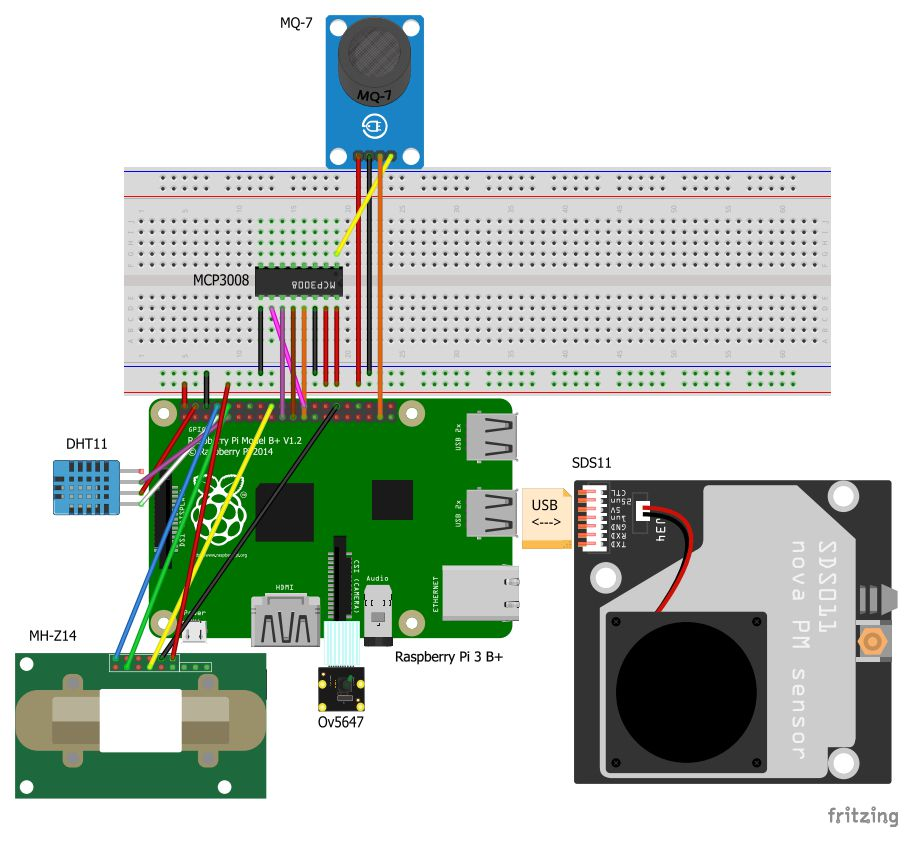
\includegraphics[width=\textwidth]{circuito.jpg}}
\end{figure}

Se comienza con los sensores con los que cuenta el dispositivo:
\begin{itemize}
	\item \textbf{DHT11}: Se trata del sensor de temperatura y humedad elegido.
	      
	      Por medio de la conexión de DATA con GPIO 4, indicada con el cable blanco, se obtiene la temperatura y la humedad del ambiente. 
	      
	      El cable rojo lo conecta con la corriente de 5 V\@.
	      
	      El cable morado lo conecta a un puerto de tierra, GND\@.
	\item \textbf{MQ-7}: Es el sensor de dióxido de carbono. Al tratarse de un sensor analógico y dado que la Raspberry no posee pines de este tipo se emplea un conversor MCP3008 que proporciona 8 canales analógicos de 10 bits.
	      
	      Se conecta mediante la protoboard a la corriente de 5 V y a tierra, cable rojo y negro respectivamente.
	      
	      En cuanto a los datos se conecta al conversor con el cable amarillo y al GPIO 26 mediante el naranja.
	      
	      El conversor se conecta a la corriente y a tierra mediante la protoboard, como el sensor, pero este además se debe conectar a los puertos SPI0\_MOSI, SPI0\_MISO, SPI0\_SCLK y SPI0\_CE0 para ofrecer los puertos analógicos. El conversor sigue el esquema de la \autoref{fig:MCP3008}~\cite{microchip_technology_inc_27v_2008} y para su uso se consulta la guía~\cite{dicola_raspberry_nodate}.
	      \begin{figure}[H]
		      \ffigbox[\FBwidth]
		      {\caption{Esquema conversor MCP3008}
			      \label{fig:MCP3008}}
		      {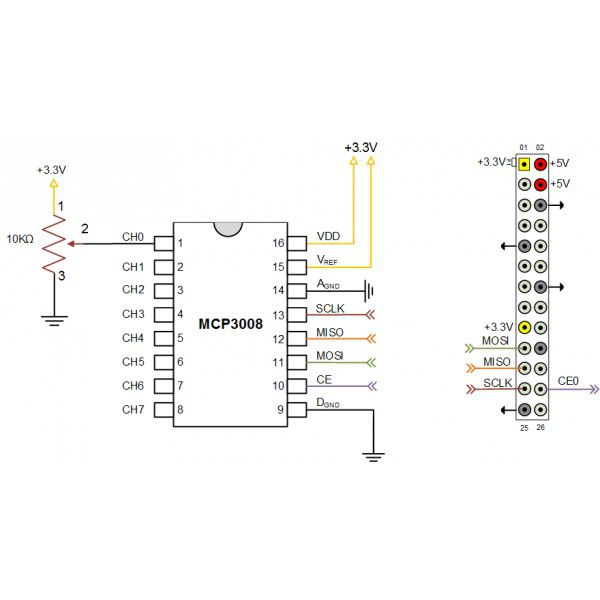
\includegraphics[scale=0.5]{mcp3008.jpg}}
	      \end{figure}
	\item \textbf{MH-Z14}: Es el sensor de CO$_2$ empleado.
	      
	      Se alimenta mediante el cable rojo a la corriente de 5 V y a tierra mediante el cable negro, ambos por medio de la protoboard. Se emplea la protoboard por falta de puertos únicos de corriente.
	      
	      Por otro lado, para transmitir los datos de las medidas utiliza los cables azul y verde a los puertos UART\_TXD y UART\_RXD respectivamente. Además, con el cable amarillo se une la salida analógica con el GPIO 24. El esquema de los pines se puede ver en la \autoref{fig:MH-Z14}~\cite{zhengzhou_winsen_electronics_technology_users_nodate}.
	      \begin{figure}[H]
		      \ffigbox[\FBwidth]
		      {\caption{Esquema del sensor MH-Z14}
			      \label{fig:MH-Z14}}
		      {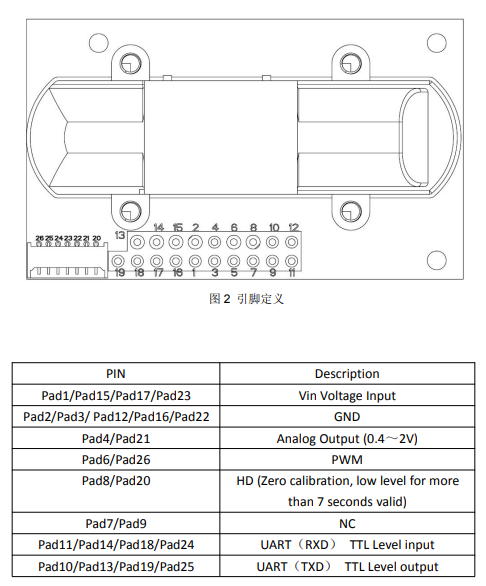
\includegraphics[scale=0.77]{MH-Z14.png}}
	      \end{figure}
	\item \textbf{SDS011}: Módulo de medida de partículas en suspensión, que se conecta mediante USB a la placa.
\end{itemize}

En cuanto a la cámara se usa la Raspberry Pi Camera, más específicamente la \textbf{Ov5647}, que se conecta mediante el puerto CSI directamente a la Raspberry Pi. Esta es la encargada de captar la imagen del CPD en el que se encuentre instalado el dispositivo.

Todas las características técnicas y el porqué de la elección de los sensores y cámara se pueden consultar en la \autoref{subsec:altComponentes}.

Como se puede ver, el elemento central es la \textbf{Raspberry Pi 3B+}, cuyas características se pueden consultar en la \autoref{subsec:altPlacas}. Además, esta se encuentra conectada a la corriente mediante un Micro USB y a la red mediante Ethernet.

Su función es alimentar y acceder a los sensores y cámara, que son los elementos que se encargan de la medición y visualización de la sala, dado que sin la Raspberry estos no serían capaces de funcionar por si solos. Otra de sus funciones clave es la retransmisión de la imagen y el envío de las medidas al servidor. Es por esta razón que se encuentra conectada a la red vía Ethernet.